\chapter{Mission: Plant}

% played on a~2'x3' play area as

\emph{\emph{Plant} is a RECON+ mission in which the alliances attempt
  to destroy the campus physical plant using explosives and targets
  chosen to incriminate the opposing side, while not being
  implicated themselves.}

\section{Play Area}
\vspace{-2\parskip}
\noindent\begin{stdminipage}{\linewidth-(2in+1.5em)}
\vspace{0pt}   
\noindent
Whichever player takes Deployment in the Initiative Roll chooses a
corner of the play area for their Deployment Zone, which extends~12''
out from that corner.  The other player takes the diagonally opposite
corner as their Deployment Zone, again extending~12'' out.

The centerline of the play area for purposes of Infiltration and other
rules is the diagonal line between the other two corners.

In Deployment order but before either player deploys, each player
places three Consoles.  One must be placed within their Deployment
Zone and the other two within their half of the play area but at least
4'' from their Deployment Zone (16'' from their corner).  None may be
placed within~4'' of the long play area edges or~6'' of the short play
area edges.  The Consoles may be placed on Buildings or other Scenery
Structures, but not in any position requiring a Climb order to reach.

A Network Terminal is placed at the center of the play area.

\section{Mission Rules}

\end{stdminipage}
\hfill
\begin{minipage}[t]{2in}\centering
\vspace{4pt}   
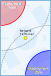
\includegraphics{maps/map-plant}
\end{minipage}

D-Charges may be placed on Consoles but the latter may not otherwise
be targeted.  As part of deployment, three troopers in each player's
army are given D-Charges.  This is public information as usual.
D-Charges already included in troopers' profiles may also be used.

\section{Scoring}

Players may score up to~10 objective points via the following
conditions at game end:
\begin{squishitemize}
\item 1pt for each enemy Console detonated with D-Charges.
\item 2pts additionally for detonating the Console in your opponent's
  Deployment Zone.
\item 1pt for each Console you placed that has not been detonated.
\item 1pt if your Special Agent is in base contact with an enemy
  Console (detonated or not).
\item 1pt if more points of the opposing army list have been destroyed.
\end{squishitemize}

\vfill
\vbox to 0pt{}